\label{sec:model}

%\begin{figure}
%\centering
%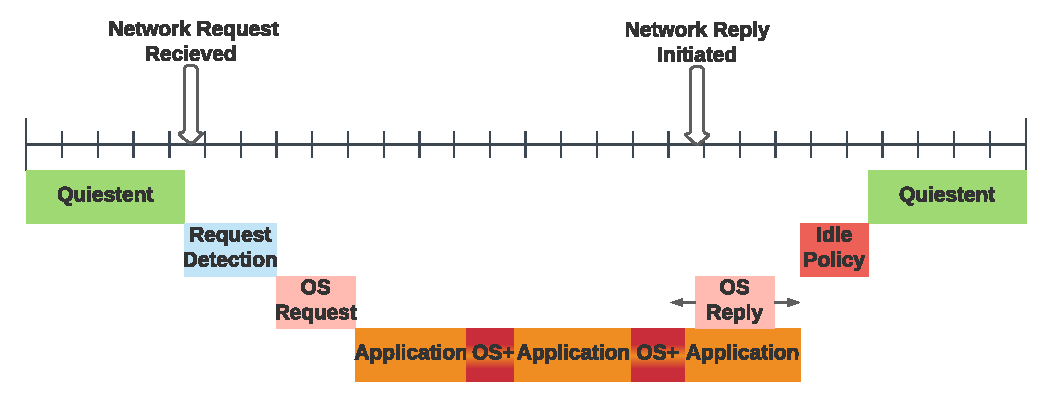
\includegraphics[width=0.5\textwidth]{figures/timeline_chart}
%\caption[]{Logical execution timeline for a single application request}
%\label{fig:timeline}
%\end{figure}

\subsection{Equations}

Using the timeline show in figure X, the total time between two consecutive requests arriving at an arrival rate can be modeled as:

$\delta t = t_{\text{detect}} + t_{\text{osref}} + t_{\text{app}} + t_{\text{idlepolicy}} + t_q$

where 

$\delta t = $ time between the arrivals of two consecutive requests

$t_{\text{detect}} = $

$t_{\text{osref}} = $

$t_{\text{app}} = $

$t_{\text{idlepolicy}} = $

$t_q = $

For a constant arrival rate and ignoring stochastic effects for a qualitative analysis, $\delta t = \frac{1}{\lambda}$ where $\lambda$ is the arrival rate. So,

$\delta t = t_{\text{detect}} + t_{\text{osref}} + t_{\text{app}} + t_{\text{idlepolicy}} + t_q = \frac{1}{\lambda}$

This implies that the quiescent time is:

$t_q = \left[\frac{1}{\lambda} - t_\text{busy}\right]^+$

where $t_{\text{busy}} \equiv t_{\text{detect}} + t_{\text{osref}} + t_{\text{app}} + t_{\text{idlepolicy}}$

and 

$[x]^+ = \max(x,0)$

i.e. $[x]^+$ is the positive part of $x$.

In other words, if the arrival rate $\lambda$ is small, there is an opportunity for the processor to enter a quiescent state ($t_q > 0$) but as the arrival rate increases, the time processing the request, $t_\text{busy}$ exceeds the inter-arrival gap leading to requests accumulating in the queue. 

This relationship also applies to the closed-loop case (Netpipe and NodeJS) with the additional constraint that the arrival rate and thus the inter-arrival gap is no longer independent of $t_\text{busy}$.

We will generally work in the regime where $t_q \geq 0$ i.e. the arrival rate is small enough that there is some opportunity to sleep if sleep states are enabled.

Given this time decomposition, one can compute the total energy consumed for each request as follows:

$E = P_\text{detect} t_{\text{detect}} + P_{\text{work}} \left[t_{\text{osref}} + t_{\text{app}} + t_{\text{idlepolicy}}\right] + P_q t_q$

where three different power regimes have been introduced:

$P_\text{detect} = $

$P_\text{work} = $

$P_q = $

We can now posit the dependence of some of the terms on DVFS.

Suppose the workload needs $N_i$ instructions. One would expect $t_\text{app}$ to scale as:

$t_{\text{app}} \propto \frac{N_i}{f}$

where $f = $ CPU frequency. Of course, there might be deviations from this behavior and one can posit a power law dependence as:

$t_{\text{app}} = A\frac{N_i}{f^{1+\alpha'}}$

where A is a constant of proportionality and $\alpha'$ is an arbitrary parameter. $\alpha'$ = 0 would fit the baseline case where time scales inversely with frequency.

Since we control DVFS and not frequency directly, we can change this to

$t_{\text{app}} = A\frac{N_i}{\Delta^{1+\alpha}}$

where DVFS = the chosen DVFS value and $\alpha$ is some scaling power that can be inferred from data. The other time values don't depend on DVFS.

The total energy consumed depends on various power values which in turn can depend on DVFS. Here, we posit that $P_{\text{work}}$ has a power law dependence on DVFS. To motivate this, the power consumed by a processor scales as:

$P \propto V^2 f$

where V = the operating voltage and f = CPU frequency. DVFS scales both voltage and frequency but not necessarily in a linear way. The general power law assumption is parameterized by a second parameter, $beta$, as follows:

$P_{\text{work}} = B \Delta^{2+\beta}$

where B is a constant of proportionality and $\beta$ can be unrestricited and is meant to be inferred from the data. Depending on the exact setup, it is possible that $P_{\text{detect}}$ also scales with DVFS and in that case, we will set $P_{\text{detect}} = P_{\text{work}}$.

At a qualitative level, the two relationships,

$\boxed{\delta t = t_{\text{detect}} + t_{\text{osref}} + t_{\text{app}} + t_{\text{idlepolicy}} + t_q}$

$\boxed{E = P_\text{detect} t_{\text{detect}} + P_{\text{work}} \left[t_{\text{osref}} + t_{\text{app}} + t_{\text{idlepolicy}}\right] + P_q t_q}$

with the requirements that:

$\delta t = \frac{1}{\lambda}$ or equivalently, $t_q = \left[\frac{1}{\lambda} - t_\text{busy}\right]^+$ with $t_{\text{busy}} \equiv t_{\text{detect}} + t_{\text{osref}} + t_{\text{app}} + t_{\text{idlepolicy}}$.

can be used to plot the behavior of energy consumed vs time (latency, total run-time) for various values of $\alpha$ and $\beta$.

%\subsection{ITR-Delay algorithm}
